\documentclass[a4paper,12pt]{article} % тип документа

%  Русский язык
\usepackage[T2A]{fontenc}			% кодировка
\usepackage[utf8]{inputenc}			% кодировка исходного текста
\usepackage[english,russian]{babel}	% локализация и переносы

\usepackage{graphicx}               % импорт изображений
\usepackage{wrapfig}                % обтекаемые изображения
\graphicspath{{pictures/}}          % обращение к подкаталогу с изображениями
\usepackage[14pt]{extsizes}         % для того чтобы задать нестандартный 14-ый размер шрифта
\usepackage{amsfonts}               % буквы с двойными штрихами
\usepackage[warn]{mathtext}         % русский язык в формулах
\usepackage{indentfirst}            % indent first
\usepackage[margin = 25mm]{geometry}% отступы полей
\usepackage{amsmath}                % можно выводить фигурные скобочки -- делать системы уравнений
\usepackage[table,xcdraw]{xcolor}   % таблицы
\usepackage{amsmath,amsfonts,amssymb,amsthm,mathtools} % Математика
\usepackage{wasysym}                % ???
\usepackage{upgreek}                % ???  

\usepackage{caption}
\captionsetup{labelsep=period}
\usepackage{gensymb} % degree symbol

\begin{document}
	\begin{center}
		
		\normalsize{Федеральное государственное автономное образовательное учреждение высшего образования}
		
		\textbf{НАЦИОНАЛЬНЫЙ ИССЛЕДОВАТЕЛЬСКИЙ УНИВЕРСИТЕТ \\ <<МОСКОВСКИЙ ФИЗИКО-ТЕХНИЧЕСКИЙ ИНСТИТУТ>>}
		\vspace{13ex}
		
		\textbf{Лабораторная работа 2.4.1 \\ <<Определение теплоты испарения жидкости>> }
		\vspace{40ex}
		
		\normalsize{Овсянников Михаил Александрович \\ студент группы Б01-001\\ 1 курс ФРКТ\\}
	\end{center}
	
	\vfill 
	
	\begin{center}
		г. Долгопрудный\\ 
		2021 г.
	\end{center}
	
	\thispagestyle{empty} % выключаем отображение номера для этой страницы
	
	\newpage
	
	\textbf{Цель работы:} измерение давления насыщенного пара жидкости при разной температуре; вычисление по полученным данным теплоты испарения с помощью уравнения Клайперона-Клазиуса.\\
	
	\textbf{В работе используются:} термостат, герметический сосуд с исследуемой жидкостью, отсчетный микроскоп.\\ 
	
	\section*{Теоретические сведения}
	Испарением называется переход вещества из жидкого в газообразное состояние. При испарении совершается работа против внешнего давления $P$, поскольку объем жидкости меньше объема пара.
	
	\indent В настоящей работе для определения теплоты испарения применен косвенный метод, основанный на формуле Клапейрона–Клаузиуса:
	
	\begin{equation} \label{уравнение Клапейрона–Клаузиуса}
		\frac{dP}{dT} = \frac{L}{T(V_{2} - V_{1})}
	\end{equation}
	
	
	\indent При нашей точности опытов величиной $V_{1}$ в (1) можно пренебречь.
	
	\indent Обратимся $V_{2}$, которое в дальнейшем будем обозначать
	просто $V$. Объем $V$ связан с давлением и температурой уравнением Ван-дер-Ваальса:
	
	\begin{equation} \label{уравнение Ван-дер-Ваальса}
		\left(P + \frac{a}{V^2}\right)(V - b) = RT
	\end{equation}
	
	\indent В уравнении \eqref{уравнение Ван-дер-Ваальса} величиной $b$ следует пренебречь, так как она одного порядка с $V_{1}$. Пренебрежение членом $\frac{a}{V^2}$ по сравнению с $P$ вносит ошибку менее 3$\%$. При давлении ниже атмосферного ошибки становятся еще меньше. Таким образом, при давлениях ниже атмосферного уравнение Ван-дер-Ваальса для насыщенного пара мало отличается от уравнения Клапейрона.
	Положим поэтому
	
	\begin{equation} \label{Клайперон}
		V = \frac{RT}{P}
	\end{equation}
	
	Подставляя \eqref{Клайперон} в \eqref{уравнение Клапейрона–Клаузиуса}, пренебрегая $V_{1}$ и разрешая уравнение относительно $L$, найдем
	
	\begin{equation}
		L = \frac{RT^2}{P}\frac{dP}{dT} = -R\frac{d(\text{ln} P)}{d(1/T)}
	\end{equation}
	
	Эта формула является окончательной.
	В нашем опыте температура жидкости измеряется термометром, давление пара определяется при помощи манометра, а производные $dP/dT$ или $d(\ln P)/d(1/T)$ находятся графически как угловой коэффициент касательной к кривой $P(T)$ или соответственно к кривой, у которой по оси абсцисс отложено $1/T$, а по оси ординат $\ln P$.
	
	\section*{Экспериментальная установка} 
	Схема установки изображена на рисунке 1. Установка включает термостат A, экспериментальный прибор B и отсчетный микроскоп C. 
	
	Наполненный водой резервуар 1 играет роль термостата. Нагревание термостата производится спиралью 2, подогреваемой электрическим током. Для охлаждения воды в термостате через змеевик 3 пропускается водопроводная вода. Вода в термостате перемешивается воздухом, поступающим через трубку 4. Температура воды измеряется термометром 5. В термостат погружен запаянный прибор 6 с исследуемой жидкостью. Над ней находится насыщенный пар (перед заполнением прибора воздух из него был откачан). Давление насыщенного пара определяется по ртутному манометру, соединенному с исследуемым объемом. Отсчет показаний манометра производится при помощи микроскопа. 
	
	\begin{figure}[h!]
		\centering
		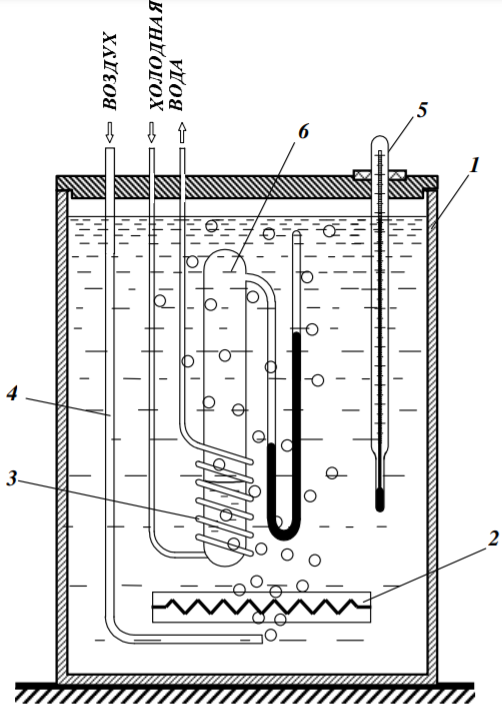
\includegraphics[scale = 0.7]{Pictures/Установка.png}
		\caption{Схема установки для определения теплоты испарения}
	\end{figure}

	\newpage
	
	\section*{Ход Работы}
	\begin{enumerate}
		\item Измерим разность уровней в ртутном $U$-образном манометре с помощью микроскопа и температуру по термометру или индикаторному табло (табл.1).
		
		\item Включим термостат. Подогреваем воду в калориметре, пропуская ток через нагреватель. Следим за тем, чтобы воздух все время перемешивал воду. Через каждый градус измеряем давление и температуру (табл.1). Продолжаем повышать температуру в течение половины имеющегося у нас времени, чтобы успеть произвести измерения при остывании прибора. Нагреваем жидкость до 38 $\degree$C.
		
		\item Проведем те же измерения при охлаждении жидкости (табл.1). Установим такой поток воды, чтобы охлаждение шло примерно тем же темпом, что и нагревание.

		
		
		\begin{table}[h!]
			\centering
			\begin{tabular}{|c|c|c|c|c|c|c|c|}
				\hline
				$T$, K & $h_{\text{лев}}$, мм & $h_{\text{конд}}$, мм & $h_{\text{прав}}$, мм & $T$, K & $h_{\text{лев}}$, мм & $h_{\text{конд}}$, мм & $h_{\text{прав}}$, мм \\ \hline
				\multicolumn{4}{|c|}{Повышение температуры}                                  & \multicolumn{4}{c|}{Повышение температуры}                                   \\ \hline
				295    & 99,8                 & 55,3                 & 57,7                  & 295    & 135,5                & 20,6                 & 23,2                  \\ \hline
				296    & 102,5                & 53,8                 & 56,7                  & 296    & 132,6                & 24,0                 & 27,0                  \\ \hline
				297    & 103,9                & 51,3                 & 54,0                  & 297    & 130,1                & 25,9                 & 29,5                  \\ \hline
				298    & 105,4                & 49,7                 & 52,6                  & 298    & 126,9                & 28,9                 & 32,2                  \\ \hline
				299    & 107,0                & 48,7                 & 51,3                  & 299    & 125,0                & 31,9                 & 34,3                  \\ \hline
				300    & 109,1                & 47,2                 & 49,6                  & 300    & 121,4                & 34,3                 & 36,9                  \\ \hline
				301    & 110,7                & 45,3                 & 47,4                  & 301    & 119,5                & 37,0                 & 39,8                  \\ \hline
				302    & 112,8                & 43,7                 & 45,5                  & 302    & 116,3                & 38,9                 & 41,9                  \\ \hline
				303    & 114,7                & 41,1                 & 44,0                  & 303    & 114,9                & 40,9                 & 44,2                  \\ \hline
				304    & 116,5                & 39,0                 & 41,7                  & 304    & 112,4                & 43,5                 & 45,2                  \\ \hline
				305    & 119,3                & 36,9                 & 39,7                  & 305    & 110,3                & 45,1                 & 47,2                  \\ \hline
				306    & 121,7                & 34,5                 & 37,1                  & 306    & 109,2                & 46,9                 & 49,3                  \\ \hline
				307    & 124,9                & 31,8                 & 34,6                  & 307    & 107,1                & 48,5                 & 51,2                  \\ \hline
				308    & 126,5                & 29,5                 & 32,2                  & 308    & 105,3                & 49,6                 & 52,3                  \\ \hline
				309    & 130,3                & 26,2                 & 29,3                  & 309    & 104,1                & 51,1                 & 53,9                  \\ \hline
				310    & 132,2                & 23,8                 & 26,9                  & 310    & 102,7                & 54,0                 & 56,9                  \\ \hline
				311    & 135,7                & 20,5                 & 23,1                  & 311    & 101,3                & 55,2                 & 57,9                  \\ \hline
			\end{tabular}
		\caption{}
		\end{table}
	
	\newpage
	\item Построим графики в координатах $T, P$.(график 1)
	\begin{figure}[h!]
		\centering
		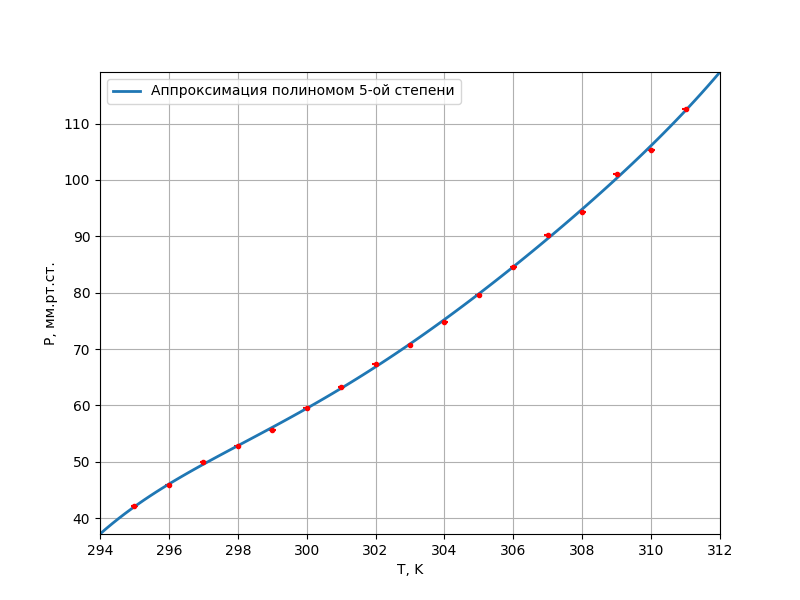
\includegraphics[scale = 0.8]{Pictures/График 1.png}
		\caption*{График 1. Повышение температуры}
	\end{figure}
	\newpage
	\begin{figure}[h!]
		\centering
		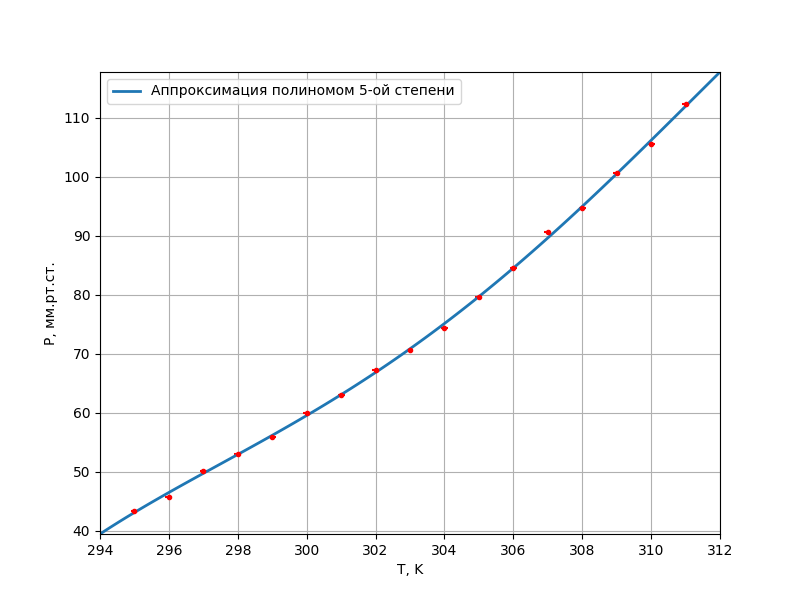
\includegraphics[scale = 0.8]{Pictures/График 2.png}
		\caption*{График 2. Понижение температуры}
	\end{figure}
	\vspace{15mm}

	Теперь построим график в координатах $\frac{1}{T}$ и $\ln{P}$ (график 3).
	
	$L = -R\frac{d(\ln{P})}{d(1/T)}$
	
	Используя МНК, находим:
	
	$k = \frac{d(\ln{P})}{d(1/T)} = -5485$ K
	
	$\sigma_{k} = 46$ K
	
	$k = (-5485 \pm 46)$ K
	\newpage
	\begin{figure}[h!]
		\centering
		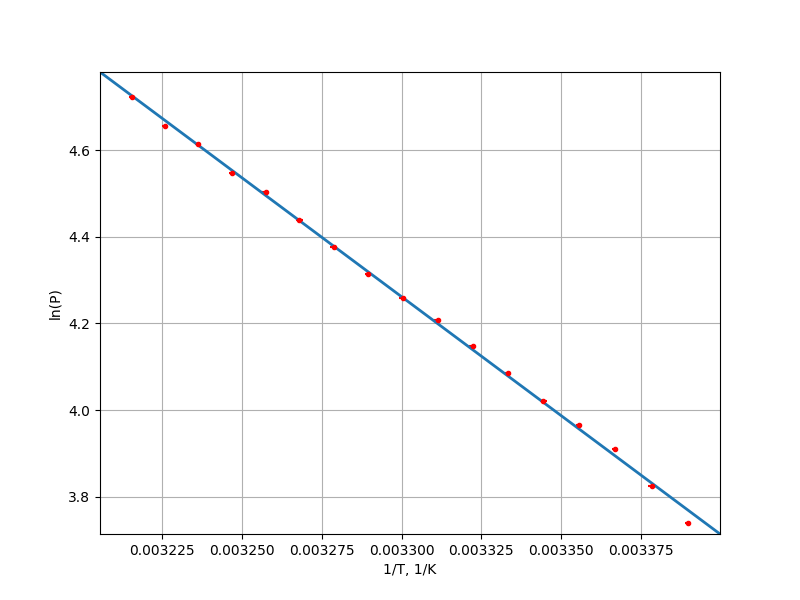
\includegraphics[scale = 0.8]{Pictures/График 3.png}
		\caption*{График 3. Повышение температуры}
	\end{figure}
	
	\vspace{15mm}
	
	Делаем то же самое для понижения температуры.
	
	Используя МНК, получаем:
	
	$k = \frac{d(\ln{P})}{d(1/T)} = -5413$ K
	
	$\sigma_{k} = 35$ K
	
	$k = (-5413 \pm 35)$ K
	\newpage
	\begin{figure}[h!]
		\centering
		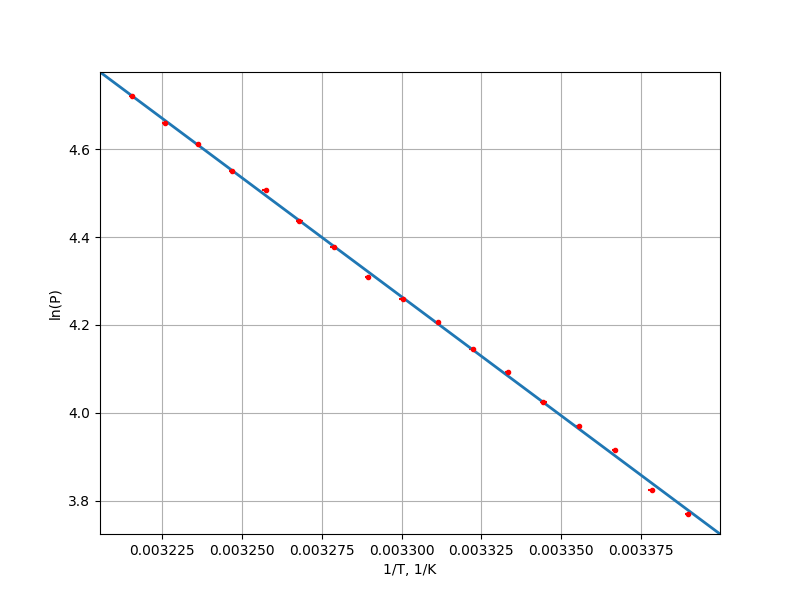
\includegraphics[scale = 0.8]{Pictures/График 4.png}
		\caption*{График 4. Понижение температуры}
	\end{figure}

	\item По формуле (4) вычислим $L$, пользуясь данными, полученными из первых двух графиков.
	
	Используя метод конечных разностей, для первого графика получаем:
	
	$L = 46114 \text{ }\frac{\text{Дж}}{\text{моль}}$
	
	$\sigma_{L} = 5239 \text{ }\frac{\text{Дж}}{\text{моль}}$
	
	$L = (46114 \pm 5239) \text{ }\frac{\text{Дж}}{\text{моль}}$
	
	\vspace{7mm}
	
	Для второго графика получаем:
	
	$L = 45416 \text{ }\frac{\text{Дж}}{\text{моль}}$
	
	$\sigma_{L} = 4324 \text{ }\frac{\text{Дж}}{\text{моль}}$
	
	$L = (45416 \pm 4324) \text{ }\frac{\text{Дж}}{\text{моль}}$
	
	\newpage
	Найдем значение $L$ для второй пары графиков.
	
	Из третьего графика находим:
	
	$L = -R \cdot k = -8.314 \cdot (-5485) \text{ }\frac{\text{Дж}}{\text{моль}} = 45602 \text{ }\frac{\text{Дж}}{\text{моль}}$
	
	$\sigma_{L} = R \sigma_{k} = 8.314 \cdot 46 \text{ }\frac{\text{Дж}}{\text{моль}} = 382 \text{ }\frac{\text{Дж}}{\text{моль}}$
	
	$L = (45602 \pm 382) \text{ }\frac{\text{Дж}}{\text{моль}}$
	
	\vspace{7mm}
	
	Из четвертого графика получаем:
	
		$L = -R \cdot k = -8.314 \cdot (-5413) \text{ }\frac{\text{Дж}}{\text{моль}} = 45004 \text{ }\frac{\text{Дж}}{\text{моль}}$
	
	$\sigma_{L} = R \sigma_{k} = 8.314 \cdot 35 \text{ }\frac{\text{Дж}}{\text{моль}} = 291 \text{ }\frac{\text{Дж}}{\text{моль}}$
	
	$L = (45004 \pm 291) \text{ }\frac{\text{Дж}}{\text{моль}}$.
	
	\vspace{20mm}

	$\hspace{40mm}L_{\text{итог}} = (45534 \pm 6809) \text{ }\frac{\text{Дж}}{\text{моль}}$.
	
	\vspace{20mm}
	Сравним результаты. Как видим, в пределах погрешностей полученные значения из всех графиков находятся в согласии друг с другом. Табличное значение для спирта: $38500-39500 \text{ }\frac{\text{Дж}}{\text{моль}}$ для этилового и $45500-46500 \text{ }\frac{\text{Дж}}{\text{моль}}$ для пропилового. Следовательно, можно предположить, что в эксперименте был пропиловый спирт с небольшими примесями. Погрешность определения $L$ составляет $\thicksim 2-7 \%$ для различных графиков. Наиболее точный результат дал график 3.
	\end{enumerate}
	\newpage
	
	\section*{Вывод}
	В работе было измерено давление насыщенного пара спирта при различных температурах. Также по полученным данным была вычислена молярная теплота испарения спирта с помощью уравнения Клайперона-Клаузиуса $L = (45534 \pm 6809) \text{ }\frac{\text{Дж}}{\text{моль}}$, что почти совпадает с табличным значением для пропилового спирта. Ошибки вызваны неточностью измерений.
\end{document}